\section{曲率的处理}
\label{sec:sqp-curvature}

式~\eqref{eq:sqp-lagrangian-hessian}的矩阵在解附近很好，远离解时却可能不定。这就需要回答：$\bm{B}^{(t)}$既要反映真实的局部曲率，又要让子问题有意义、让步能被接受，这两者怎样兼顾？

\paragraph{KKT系统可解不等于模型是碗}
先把两件容易混淆的事分开。设只有一条约束$d_2=0$，即$\bm{A}=(0,1)$，线性项$\bm{c}=(-0.6,0.3)^\top$，比较三个矩阵：
\[
 \bm{B}_a=\begin{bmatrix}1&0\\0&1\end{bmatrix},\qquad
 \bm{B}_b=\begin{bmatrix}1&0\\0&-1\end{bmatrix},\qquad
 \bm{B}_c=\begin{bmatrix}-1&0\\0&1\end{bmatrix}.
\]

这里零空间由$\bm{e}_1$张成，约化Hessian就是左上角的元素。三种情形下KKT矩阵都可逆，解都由$B_{1,1}d_1=0.6$给出，对应的$\bm{d}$分别是
\[
 (0.6,\ 0)^\top,\qquad(0.6,\ 0)^\top,\qquad(-0.6,\ 0)^\top.
\]

图~\ref{fig:sqp-kkt-vs-convexity}是这三个模型。情形(a)是凸的，解是最小点。情形(b)的$\bm{B}$不定，整个二次目标不是凸的，可是沿约束直线它向上弯，解仍是约束上的最小点。情形(c)的$\bm{B}$同样不定，沿直线却向下弯，解是约束上的最大点，模型沿直线无下界。

\begin{BookInlineFigure}
 \centering
 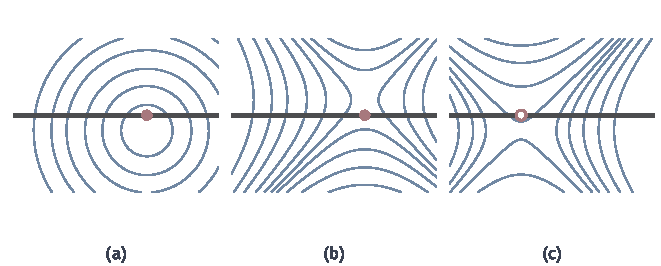
\includegraphics[width=112mm]{figures/05-optimization/06-constrained-optimization/matplotlib/sqp-kkt-vs-convexity/figure.pdf}
 \caption{三个KKT矩阵都可逆的模型，蓝线是二次目标的等高线，深灰粗线是约束$d_2=0$。(a)~$\bm{B}$正定，解（红点）是最小点。(b)~$\bm{B}$不定而约化Hessian为正，解仍是约束上的最小点。(c)~约化Hessian为负，KKT系统的解（空心点）是约束上的最大点。}
 \label{fig:sqp-kkt-vs-convexity}
\end{BookInlineFigure}

所以有三个不同的判断：KKT矩阵可逆；约化Hessian正定；$\bm{B}$在全空间正定。第三个推出第二个，第二个在行满秩时推出第一个，反过来都不成立。整个二次目标凸不凸，本身不是SQP需要的条件。

这几件事可以通过分解读出来。矩阵的\term{惯性}（inertia）是其正、负、零特征值的个数。$\bm{A}$行满秩时可以证明，$\bm{K}$的惯性等于$\bm{Z}^\top\bm{B}\bm{Z}$的惯性再各加上$p$个正、负特征值，证明要用一次合同变换，篇幅不长，读者可查阅专著\scite{math-nocedal2006numerical}。因此约化Hessian正定当且仅当$\bm{K}$恰有$n$个正特征值和$p$个负特征值。

用上面三个矩阵核对。这里$n=2$，$p=1$，$\bm{K}_a$和$\bm{K}_b$的惯性都是$(2,1,0)$；$\bm{K}_c$的特征值是$-1$和$(1\pm\sqrt5)/2$，惯性是$(1,2,0)$，多出一个负特征值，正好标记了错误的曲率。

子问题由什么方法求解，决定了实际要满足什么。表~\ref{tab:sqp-curvature-needs}按求解器列出要求。

\begin{BookInlineTable}
 \centering
 \begin{tabular}{ll}
  \toprule
  子问题的解法 & 对$\bm{B}$的实际要求\\
  \midrule
  直接解KKT系统 & 可逆即可解，是否最小点要另查惯性\\
  零空间方法 & 约化Hessian正定\\
  有效集法 & 每个工作集的约化Hessian正定\\
  要求凸QP的内点法等 & 通常要求$\bm{B}$半正定\\
  \bottomrule
 \end{tabular}
 \caption{不同子问题解法对曲率的要求。}
 \label{tab:sqp-curvature-needs}
\end{BookInlineTable}

\subsection{Hessian修正}
\label{sec:sqp-hessian-modification}

\paragraph{负曲率的例子}
乘子估计差得远时，精确的$\bm{B}$就可能是错的。回到问题~\eqref{eq:sqp-circle}的$\bm{x}^{(0)}=(1.5,0.5)^\top$，把乘子估计错成$\nu=-1$，于是$\bm{B}=2\nu\bm{I}=-2\bm{I}$，在任何方向上都向下弯。

KKT系统依然可解。第一行是$-2\bm{d}+\bm{g}+\hat\nu\bm{A}^\top=\bm{0}$，由此
\[
 \bm{d}=\frac12\bigl(\bm{g}+\hat\nu\bm{A}^\top\bigr)=\frac12\begin{bmatrix}3\hat\nu-1\\\hat\nu-1\end{bmatrix}.
\]

代入第二行$\bm{A}\bm{d}=-0.5$，左端是$5\hat\nu-2$，于是
\[
 \hat\nu=0.3,\qquad\bm{d}=(-0.05,\ -0.35)^\top.
\]

这个步是否合用，要沿线性化约束看模型。把允许的步写成$\bm{d}=\bm{d}_Y+s\bm{t}$，其中$\bm{d}_Y=(-0.15,-0.05)^\top$是第~\ref{sec:sqp-equality-qp}节的法向段，$\bm{t}=(-1,3)^\top/\sqrt{10}$是虚线的单位方向。代入模型并利用$\bm{d}_Y\perp\bm{t}$，得到
\[
 q(s)=0.175-0.632\,s-s^2.
\]

上式对$s$向下弯，模型沿线性化约束没有下界。KKT系统给出的$\bm{d}$对应$s\approx-0.316$，正是图~\ref{fig:sqp-curvature-repair}红线的最高点。求解这个方程得到的是模型的最大点，把它当作下降步是错的。

\begin{BookInlineFigure}
 \centering
 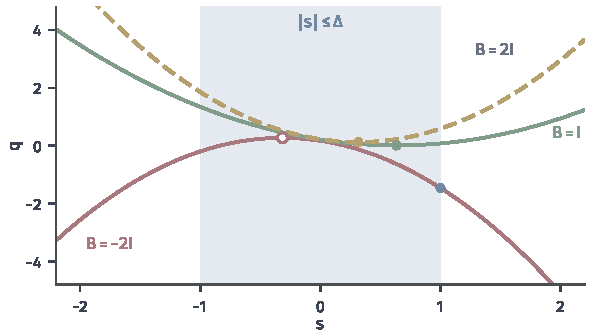
\includegraphics[width=100mm]{figures/05-optimization/06-constrained-optimization/matplotlib/sqp-curvature-repair/figure.pdf}
 \caption{沿线性化约束的模型$q(s)$，$s$是沿虚线方向的位移。红线是$\bm{B}=-2\bm{I}$，空心点是KKT系统的解，它是最大点。绿线、黄色虚线是移位后的$\bm{B}=\bm{I}$与$\bm{B}=2\bm{I}$，圆点是各自的最小点。浅蓝带是信赖域$\lvert s\rvert\leq\Delta=1$，蓝点是原模型在带内的最小点。}
 \label{fig:sqp-curvature-repair}
\end{BookInlineFigure}

\paragraph{先核对模型是否无界}
含不等式时情况稍有不同。不等式可能把下降方向挡住，QP于是有解，可是解落在边界上，是负曲率推过去的，未必是好步。所以出现负曲率时要回答两个问题：子问题本身有没有下界，以及当前这个步是否适合接受。处理的办法有三类，它们改变的东西不同。

\paragraph{移位}
第一种办法是把$\bm{B}$换成$\bm{B}+\tau\bm{I}$，这是第~\ref{chap:second-order-methods}章修正Newton法的直接推广。取$\tau$从小到大试，每次分解后检查惯性，直到约化Hessian正定。例中约化Hessian是$-2$，需要$\tau>2$。

取$\tau=3$，就是$\bm{B}=\bm{I}$。解KKT系统，第一行给$\bm{d}=(1-3\hat\nu,1-\hat\nu)^\top$，第二行给$4-10\hat\nu=-0.5$，于是
\[
 \hat\nu=0.45,\qquad\bm{d}=(-0.35,\ 0.55)^\top.
\]

移位改的是模型本身，而且改的是所有方向的曲率。$\tau$越大，步越短、越偏向梯度方向。例中$\tau=4$时步变成$(-0.25,0.25)^\top$，图~\ref{fig:sqp-curvature-repair}的黄线最低点比绿线更靠近$s=0$，就是这个效果。

\paragraph{约化曲率修正}
第二种办法只动约化Hessian。在式~\eqref{eq:sqp-reduced-step}中，把$\bm{Z}^\top\bm{B}\bm{Z}$换成一个正定矩阵，比如把负特征值取绝对值，其他量不变。例中用$\lvert-2\rvert=2$，右端不变，得到
\[
 s=\frac{0.632}{2}=0.316,\qquad\bm{d}=(-0.25,\ 0.25)^\top.
\]

这里结果恰好和$\tau=4$相同，因为$\bm{d}_Y$与$\bm{t}$正交，$\bm{B}$又是单位阵的倍数。一般两者不同：约化修正不改变法向段，也保留了$\bm{B}$在约束法方向上的信息。

\paragraph{信赖域限制}
第三种办法不改模型，而是限制步能走多远，这是第~\ref{chap:trust-region}章的想法。例中加$\lvert s\rvert\leq\Delta=1$，模型在带内的最小点在边界$s=1$，那里的模型值是$-1.457$，另一端$s=-1$的模型值是$-0.193$。

信赖域的好处是负曲率不用消除，它甚至被用来走得更远。约束优化中要多注意一件事：线性化约束和信赖域可能相互矛盾，它们的交集可能是空的。常见的处理是先取法向段，要求它只占信赖域的一部分，再在剩下的范围内取切向段。

\begin{BookInlineTable}
 \centering
 \begin{tabular}{lll}
  \toprule
  做法 & 改变了什么 & 代价或风险\\
  \midrule
  移位$\bm{B}+\tau\bm{I}$ & 所有方向的曲率 & 反复分解，步偏向梯度\\
  约化曲率修正 & 零空间内的曲率 & 需要显式的$\bm{Z}$\\
  信赖域 & 允许的步长范围 & 约束可能不相容\\
  \bottomrule
 \end{tabular}
 \caption{处理负曲率的三类办法。}
 \label{tab:sqp-modification}
\end{BookInlineTable}

这些办法各自改变了模型或步长范围。一个可解的KKT系统本身不能保证解是极小步，判断的依据只能是约化曲率或惯性。修正后的步还要经过第~\ref{sec:sqp-acceptance}节的检验。

\subsection{拟Newton近似}
\label{sec:sqp-quasi-newton}

精确的式~\eqref{eq:sqp-lagrangian-hessian}要求所有$m+p+1$个函数的二阶导数，这常常是SQP最贵也最难编写的一部分。第~\ref{chap:quasi-newton}章的办法是从梯度之差积累曲率。本小节要解决的问题是：在约束问题上，这个差该怎么取，又该怎样保持近似矩阵可用？

\paragraph{割线信息}
要近似的是Lagrange函数对$\bm{x}$的Hessian，所以差分的对象是Lagrange梯度。两点必须用同一组乘子，否则差分中混入乘子的变化，就不再是对$\nabla^2_{\bm{x}\bm{x}}\mathcal{L}$的测量。取新的乘子估计，令
\begin{equation}
 \begin{aligned}
 \bm{s}^{(t)}&=\bm{x}^{(t+1)}-\bm{x}^{(t)},\\
 \bm{y}^{(t)}&=\nabla_{\bm{x}}\mathcal{L}(\bm{x}^{(t+1)},\bm{\lambda}^{(t+1)},\bm{\nu}^{(t+1)})
 -\nabla_{\bm{x}}\mathcal{L}(\bm{x}^{(t)},\bm{\lambda}^{(t+1)},\bm{\nu}^{(t+1)}).
 \end{aligned}
 \label{eq:sqp-secant-pair}
\end{equation}

BFGS更新的公式与第~\ref{chap:quasi-newton}章相同，这里省去上标，新矩阵记作$\bm{B}^{+}$：
\begin{equation}
 \bm{B}^{+}=\bm{B}-\frac{\bm{B}\bm{s}\bm{s}^\top\bm{B}}{\bm{s}^\top\bm{B}\bm{s}}+\frac{\bm{y}\bm{y}^\top}{\bm{s}^\top\bm{y}}.
 \label{eq:sqp-bfgs}
\end{equation}

例中取第一步$\bm{s}=(-0.25,0.25)^\top$，$\hat\nu=0.5$，初始矩阵$\bm{B}=2\bm{I}$。这时Lagrange梯度是$\bm{x}-(1,1)^\top$，由它在两点之差得到
\[
 \bm{y}=\bm{s}=(-0.25,\ 0.25)^\top,\qquad\bm{s}^\top\bm{y}=0.125,\qquad\bm{s}^\top\bm{B}\bm{s}=0.25.
\]

代入式~\eqref{eq:sqp-bfgs}，并用$\bm{B}\bm{s}=2\bm{s}$，修正项化成$\bm{s}\bm{s}^\top$的倍数：
\[
 \bm{B}^{+}=2\bm{I}-16\,\bm{s}\bm{s}^\top+8\,\bm{s}\bm{s}^\top
 =\begin{bmatrix}1.5&0.5\\0.5&1.5\end{bmatrix}.
\]

可以核对割线条件$\bm{B}^{+}\bm{s}=\bm{y}$：沿$\bm{s}$的曲率从$2$变成了真实的$1$，与$\bm{s}$正交的方向仍保持$2$，因为这一次测量对那个方向没有提供信息。

\paragraph{曲率条件与阻尼}
无约束时，Wolfe线搜索能保证$\bm{s}^\top\bm{y}>0$。约束问题却不同，$\nabla^2_{\bm{x}\bm{x}}\mathcal{L}$在解处也可能是不定的，这时走出来的$\bm{s}$可能真的带着负曲率，不能靠步长选取来排除。如果$\bm{s}^\top\bm{y}\leq0$，式~\eqref{eq:sqp-bfgs}会毁掉正定性。

\term{阻尼BFGS}（damped BFGS）把$\bm{y}$换成它和$\bm{B}\bm{s}$的一个组合$\bm{r}$，组合比例只在测量不够好时才起作用：
\begin{equation}
 \begin{gathered}
 \bm{r}=\theta\bm{y}+(1-\theta)\bm{B}\bm{s},\\
 \theta=\begin{cases}
 1, & \bm{s}^\top\bm{y}\geq0.2\,\bm{s}^\top\bm{B}\bm{s},\\
 \dfrac{0.8\,\bm{s}^\top\bm{B}\bm{s}}{\bm{s}^\top\bm{B}\bm{s}-\bm{s}^\top\bm{y}}, & \text{否则}.
 \end{cases}
 \end{gathered}
 \label{eq:sqp-damped}
\end{equation}
然后在式~\eqref{eq:sqp-bfgs}中用$\bm{r}$代替$\bm{y}$。

第二种情形的$\theta$恰好使$\bm{s}^\top\bm{r}=0.2\,\bm{s}^\top\bm{B}\bm{s}>0$。把$\theta$代入即可验证：
\[
 \bm{s}^\top\bm{r}=\bm{s}^\top\bm{B}\bm{s}+\theta\bigl(\bm{s}^\top\bm{y}-\bm{s}^\top\bm{B}\bm{s}\bigr)=\bm{s}^\top\bm{B}\bm{s}-0.8\,\bm{s}^\top\bm{B}\bm{s}.
\]

所以更新后的矩阵总保持正定。图~\ref{fig:sqp-damped-rule}按上例的$\bm{s}^\top\bm{B}\bm{s}=0.25$画出这条规则。设乘子为负，真实曲率是$-2$，即$\bm{y}=-2\bm{s}$，$\bm{s}^\top\bm{y}=-0.25$，于是
\[
 \theta=\frac{0.8\times0.25}{0.25+0.25}=0.4,\qquad\bm{r}=0.4\bm{s}.
\]

沿$\bm{s}$的曲率更新后是$0.05/0.125=0.4$，即$\bm{s}^\top\bm{r}$除以$\bm{s}^\top\bm{s}$。它既不是测量到的$-2$，也不是原来的$2$。阻尼的代价是割线条件不再成立，矩阵不再记录真实的负曲率。

\begin{BookInlineFigure}
 \centering
 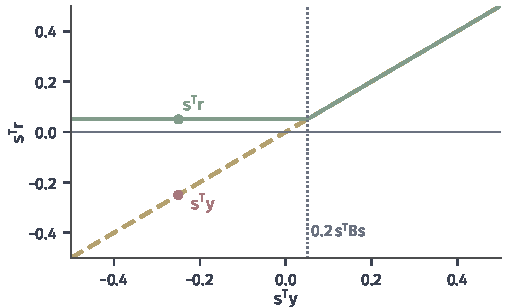
\includegraphics[width=86mm]{figures/05-optimization/06-constrained-optimization/matplotlib/sqp-damped-rule/figure.pdf}
 \caption{阻尼规则，$\bm{s}^\top\bm{B}\bm{s}=0.25$。黄色虚线是未加处理的$\bm{s}^\top\bm{y}$，绿线是阻尼后的$\bm{s}^\top\bm{r}$，它在虚线竖线以左被托在$0.2\,\bm{s}^\top\bm{B}\bm{s}=0.05$。红点是测量值$-0.25$，绿点是阻尼后的$0.05$。}
 \label{fig:sqp-damped-rule}
\end{BookInlineFigure}

\paragraph{成本与速度}
下面比较两种选择。精确Hessian每轮要算$m+p+1$个Hessian，但步是Newton型的，轮数少。拟Newton只需要梯度，却维护一个稠密的$n\times n$矩阵，破坏了$\bm{K}$可能具有的稀疏结构，这时可以改用有限记忆的表示。

图~\ref{fig:sqp-exact-bfgs-rate}是一个五变量问题上的比较，目标与约束为
\[
 \begin{gathered}
 f=\exp(x_1x_2x_3x_4x_5)-\tfrac12(x_1^3+x_2^3+1)^2,\\
 h_1=\lVert\bm{x}\rVert_2^2-10,\quad h_2=x_2x_3-5x_4x_5,\quad h_3=x_1^3+x_2^3+1.
 \end{gathered}
\]
从$(-1.8,1.7,1.9,-0.8,-0.8)^\top$与最小二乘乘子出发，精确Hessian的全步法$4$轮将误差降到$10^{-11}$以下；阻尼BFGS（$\bm{B}^{(0)}=\bm{I}$，罚函数回溯，第~\ref{sec:sqp-merit}节）前$18$轮都在攒曲率信息，步长常被缩短，之后几轮迅速下降，共需约$21$轮。

\begin{BookInlineFigure}
 \centering
 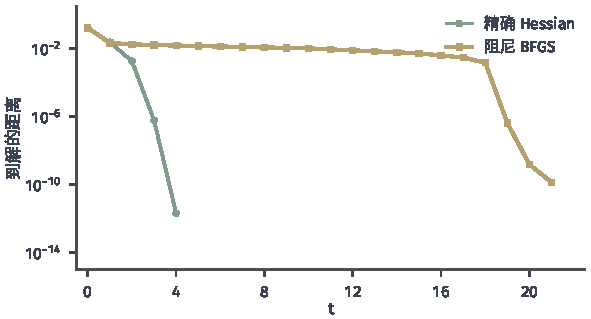
\includegraphics[width=100mm]{figures/05-optimization/06-constrained-optimization/matplotlib/sqp-exact-bfgs-rate/figure.pdf}
 \caption{五变量问题上到解的距离。绿线是精确Lagrange Hessian的全步长SQP，黄线是阻尼BFGS加罚函数回溯。两者起点相同，后者每轮不需要二阶导数。}
 \label{fig:sqp-exact-bfgs-rate}
\end{BookInlineFigure}

这个对比只是一个例子，轮数的差距随问题而变。局部速度的结论还需要曲率近似的条件。记$\bm{P}^{(t)}$是向$\bm{A}^{(t)}$零空间的投影，$\bm{H}_{\mathcal{L}}^\star$是Lagrange函数在解处对$\bm{x}$的Hessian，需要的条件是
\begin{equation}
 \lim_{t\to\infty}\frac{\lVert\bm{P}^{(t)}\bigl(\bm{B}^{(t)}-\bm{H}_{\mathcal{L}}^\star\bigr)\bm{d}^{(t)}\rVert_2}{\lVert\bm{d}^{(t)}\rVert_2}=0.
 \label{eq:sqp-dennis-more}
\end{equation}
它只要求沿步的方向、在切空间内近似准确，不要求$\bm{B}^{(t)}$收敛到真实的Hessian。这一点很重要，因为$\bm{H}_{\mathcal{L}}^\star$可以不定，而正定的BFGS矩阵无法趋于不定矩阵；在切空间上$\bm{H}_{\mathcal{L}}^\star$却是正定的，式~\eqref{eq:sqp-dennis-more}仍可能成立。
